\documentclass[xcolor=pdftex,dvipsnames,table,aspectratio=169]{beamer}
%\documentclass[xcolor=pdftex,dvipsnames,table,handout,aspectratio=169]{beamer}

%\setbeameroption{show notes}

\usepackage{bm,graphicx,multirow,amsmath,tikz} %fancybox,
\usepackage{color}%,textpos}
\usepackage[round]{natbib}
\usepackage[normalem]{ulem}
\usepackage{hyperref}
\usepackage{lastpage}
\usepackage{array}
\usepackage{color}
\usepackage{framed}
\usepackage{hyperref}

% Define Western colours
\definecolor{western}{rgb}{.306,.152,.524}
\definecolor{westerngray}{rgb}{.512,.508,.524}

%% Define BEAMER colours
\setbeamercolor{frametitle}{bg=western,fg=white}
\setbeamercolor{framesubtitle}{bg=western,fg=black}
\setbeamercolor{title}{fg=white,bg=western}
\setbeamercolor{author}{fg=white,bg=western}
\setbeamercolor{institute}{fg=white,bg=western}
\setbeamercolor{date}{fg=white,bg=western}

%% Set BEAMER fonts
\setbeamerfont{title}{shape=\bf}
\setbeamerfont{frametitle}{shape=\sc,size=\Large}
\setbeamerfont{framesubtitle}{shape=\sc,size=\Large}
\setbeamerfont{footline}{shape=\sc}

%% Define BEAMER toc
\setbeamercolor{section in toc}{fg=western}
\setbeamercolor{subsection in toc}{fg=westerngray}
\setbeamertemplate{sections/subsections in toc}[ball]

%% Define BEAMER background
\setbeamercolor{background canvas}{bg=white}

%% Define BEAMER footer
\setbeamertemplate{navigation symbols}{}
\setbeamercolor{footline}{fg=white,bg=western}
\setbeamertemplate{footline}{%
  \begin{beamercolorbox}[wd=\paperwidth]{footline}
    \vskip5pt

    \raisebox{.05in}{
      \scriptsize{\bf \insertshorttitle}
    }
    \hfill
    \raisebox{.05in}{
      \scriptsize{\bf \insertframenumber/\inserttotalframenumber} 
    }
    \hspace{5pt}

    \vskip5pt
  \end{beamercolorbox}
}

%% Define BLOCK environment
\setbeamercolor{block title}{fg=western}
\setbeamerfont{block title}{series=\bfseries}

%% Define ENUMERATE and ITEMIZE environements
\setbeamertemplate{itemize item}[ball]
\setbeamertemplate{enumerate item}[ball]
\setbeamercolor{item projected}{bg=western}

%% Define BEAMER toc
\setbeamercolor{sections/subsections in toc}{fg=blue!75}
\setbeamertemplate{sections/subsections in toc}[ball]

% %% Define SECTION openings
% \AtBeginSection[]{
%   \begin{frame}{\insertshorttitle}
%     \tableofcontents[currentsection,subsectionstyle=hide/hide/hide]
    
%   \end{frame}
% }

%% Define BEAMER frametitle
\addtobeamertemplate{frametitle}{
   \let\insertframetitle\insertsectionhead}{}
\addtobeamertemplate{frametitle}{
   \let\insertframesubtitle\insertsubsectionhead}{}


\makeatletter
  \CheckCommand*\beamer@checkframetitle{\@ifnextchar\bgroup\beamer@inlineframetitle{}}
  \renewcommand*\beamer@checkframetitle{\global\let\beamer@frametitle\relax\@ifnextchar\bgroup\beamer@inlineframetitle{}}
\makeatother

% Define counters for example and exercise
\newcounter{example}
\newcounter{exercise}

% Define example and exercise commands
\renewcommand{\example}
{\stepcounter{example}Example \lecturenum.\arabic{example}}
\newcommand{\examplectd}
{Example \lecturenum.\arabic{example}\ ctd}
\newcommand{\exercise}
{\stepcounter{exercise}Exercise \lecturenum.\arabic{exercise}}
\newcommand{\exercisectd}
{Exercise \lecturenum.\arabic{exercise}\ ctd}

\newcommand{\lecturenum}{24}

\title[SS2857]{Probability and Statistics I}
\subtitle{\lecturenum.~Statistics and their Distributions}

\date{}

%% Add logo
%% \titlegraphic{\includegraphics[height=2cm]{../uwo_logo_reversed}}

%% Initialize R


\begin{document}

{
\setbeamertemplate{footline}{}
\setbeamercolor{background canvas}{bg=western}

\begin{frame}
  \addtocounter{framenumber}{-1}

  \maketitle
\end{frame}
}

\section{Statistics and their Distributions}

\begin{frame}
  \frametitle{\invisible{Hello}}
  
  \begin{center}
    \Large{\textbf{6.1 Statistics and their Distributions}}

    \bigskip

    % \begin{center}
    %   \includegraphics[height=.5\textheight]{nestle-smarties-candies}
    % \end{center}
  \end{center}
  
\end{frame}


\begin{frame}

  \begin{center}
    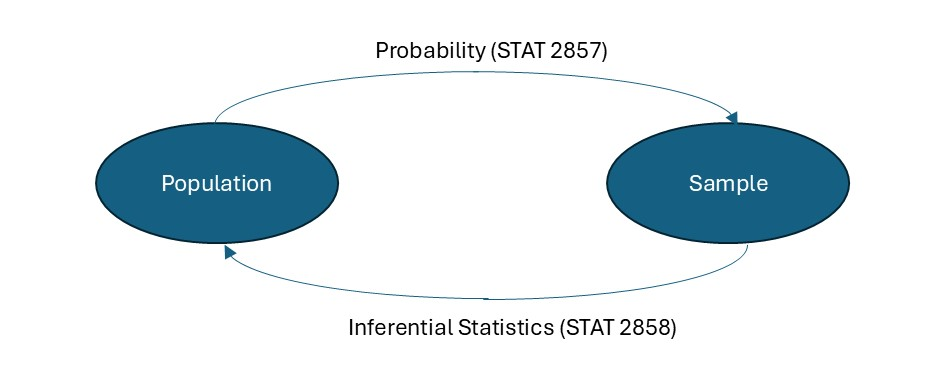
\includegraphics[height=.6\textheight]{statistics_vs_probability}
  \end{center}
\end{frame}

\begin{frame}
  \begin{block}{Statistic}
    A statistic is any quantity whose value can be calculated from sample data.

    \pause

    \bigskip

    \begin{center}
      Statistics are random variables.
    \end{center}
  \end{block}
\end{frame}

\begin{frame}
  \begin{block}{Sampling Distribution}
    The sampling distribution is the probability distribution of a statistic.

    \bigskip
    
    \begin{center}
      We use this term to highlight the fact that it is the distribution we expect to see if we repeatedly sampled many, many, many times.
    \end{center}
  \end{block}
\end{frame}

\begin{frame}
  \begin{block}{Sampling}
  There is an entire field within statistics that considers how to sample from a population to ensure that the observations are representative (SS3843A: Introduction to Study Design).
  \end{block}
\end{frame}

\begin{frame}
  \begin{block}{Random Sample}
    The random variables $X_1,\ldots,X_n$ form a random sample of size $n$ if
    \begin{enumerate}
    \item The $X_i$s are mutually independent.
    \item Every $X_i$ has the same probability distribution.
    \end{enumerate}

    \bigskip
    We also say that the $X_i$s are independent and identically distributed or \textit{iid}.
  \end{block}
\end{frame}

\begin{frame}

  \begin{block}{\example}
    The website
    \begin{center}
      \href{https://www.roulettesimulator.net/}{www.roulettesimulator.net/}
    \end{center}
    provides a free roulette simulator. Playing in free mode we can make bets in the fictional FUN currency starting with a balance of FUN 5000.
    
    \medskip
    
    I believe that the simulator may be rigged in free mode so that players win more often than they should -- possibly prompting them to "Play for Real Money".
    \end{block}
\end{frame}

\begin{frame}

  \begin{block}{\examplectd}
  Spin the wheel at \href{https://www.roulettesimulator.net/}{www.roulettesimulator.net/} 5 times placing FUN 1000 bets on black each time. Enter your final balance in the spreadsheet  \href{https://uwoca-my.sharepoint.com/:x:/g/personal/sbonner6_uwo_ca/Ee3I7Ds8g81In0-dQO_MD60BbE2CyrRa_XifWRR55PMDxw?e=uXgrB5}{here}.
    
    \begin{enumerate}[a)]
    \item Describe the simulated distribution for the balance.
      
    \item What are some statistics you could compute from our sample?
    \end{enumerate}
  \end{block}
\end{frame}

\begin{frame}

  \begin{block}{\example}
    For student $i$ denote:
    \begin{itemize}
    \item Number of wins: $X_i \sim \mbox{Binomial}(5,18/37)$
    \item Final balance: $W_i=5000+1000X - 1000(5-X)=2000X_i$.
    \end{itemize}
    
    The average balance over all students is
    $$
    \bar W=\left(\sum_{i=1}^n W_i\right)/n.
    $$

    \begin{enumerate}[a)]
    \item What is the sampling distribution of $\bar W$ if the simulator is realistic?
    \item What are the mean and variance of $\bar W$?
    \item Do you think the simulator is realistic?
    \end{enumerate}
  \end{block}
\end{frame}

\begin{frame}

  \begin{center}
    \Large{\textbf{Questions?}}
  \end{center}
\end{frame}

\begin{frame}

  \begin{block}{\exercise}
  Suppose that each student spun the wheel on the online roulette simulator betting on black repeatedly until they had won 5 times. Let $X_i$ be the number of times that the $i$-th student played and 
  $$
  \bar X = \frac{\sum_{i=1}^n X_i}{n}  
  $$
  be the average number of times played per student. 
  
  \begin{enumerate}[a)]
    \item What is the sampling distribution of $\bar X$ if the simulator is realistic?
    \item What are the mean and variance of $\bar X$?
    \item How could you use the sample values to determine if the simulator is realistic?
    \end{enumerate}
  \end{block}
\end{frame}
\end{document}
